\documentclass{article}
\title{CSC301 HW10}
\author{Alex Zhang}
\date{April 2023}
\textwidth=16.00cm 
\textheight=22.00cm 
\topmargin=0.00cm
\oddsidemargin=0.00cm 
\evensidemargin=0.00cm 
\headheight=0cm 
\headsep=0.5cm
\textheight=610pt
\usepackage{graphicx}
\usepackage{multicol}

\graphicspath{ {./images/} }

\usepackage{latexsym,array,delarray,amsthm,amssymb,epsfig}
\usepackage{amsmath}
\usepackage{listings}
\lstset{
  basicstyle=\ttfamily,
  mathescape
}

\newcommand{\bmat}[1]{\begin{bmatrix} #1 \end{bmatrix}}
\newcommand{\mat}[1]{\mathbf{#1}}

\let\ds\displaystyle

\begin{document}
\maketitle

\section*{Question 1}

Assume there is an $independent$ $set$ $S$ which in $G$. For any edge $e = (u,v)$. Only one of $u$, $v$ can be in
$S$. This means at least one of $u$, $v$ will be in $V$\textbackslash$S$ which means any $e$ is adjacent to some vertex in  vertex cover $C$.
This indicates that for given $S$ in $G$. $V$\textbackslash$S$ is the vertex cover $C$.

Assume there is a $vertex$ $cover$ $C$ that is $V$\textbackslash$S$ for a set of vertices $S$. All vertices in $S$ will not have an edge connect with 
each other or it will be in $V$\textbackslash$S$. Therefore, this means set $S$ is an $independent$ $set$ by definition.

This indicates that the sum of the number of vertices in $vertex$ $cover$ and $independent$ $set$ will be the total number of vertices.

\subsection*{(a)}
With given instance of given $G$ and $k$, we define f to change $k$ be $n-k$, where $n$ is the total number
of vertices.

Suppose we have already had an efficient algorithm to check whether $G$ has a $vertex$ $cover$ with size $\leq n-k$. 
Based on the relation of $S$ and $V$\textbackslash$S$ we showed at the beginning, h is now just doing calculation of $n-(n-k)$.
Both f and h are in polynomial time because all about is counting the number of vertices in $G$.

Based on the efficient algorithm, if there exists a $vertex$ $cover$ with size $\leq n-k$, this implies that there is an $independent$ $set$ that has size
$\geq k$, since the size of $independent$ $set$ add size of $vertex$ $cover$ is the number of vertices in $G$.

If there does not exist a $vertex$ $cover$ with size $\leq n-k$, then there is no $independent$ $set$ with size greater than $k$.

This indicates that $vertex$ $cover$ problem can be reduced into $independent$ $set$ problem. $\blacksquare$

\subsection*{(b)}
This time we define f to change $l$ to $n-l$.

Assume we have an efficient algorithm that check whether $independent$ $set$ has size $\geq n-l$. We can also define h be calculating $n - (n-l)$. both 
f and h are in polynomial time because counting the number of vertices will not cost so much time.

Based on the algorithm, if it is true, then there exists an $independent$ $set$ with size $\geq n-l$. This means that there exists a $vertex$ $cover$ with size 
$\leq l$ based on h. If it is false, then there is no $independent$ $set$ with size $\geq n-1$. This also means there is no $vertex$ $cover$ with size 
$\leq l$ because if $S$ is an $independent$ $set$ ,  $V$\textbackslash$S$ is a $vertex$ $cover$.

This shows that $independent$ $set$ problem can be reduced into $vertex$ $cover$ problem.$\blacksquare$

Overall $independent$ $set$ problem can be reduced to $vertex$ $cover$ problem and vise versa. If we just know one efficient algorithm, we can use it to solve 
two questions at the same time.



\section*{Question 2}
Since we proved that SAT $\rightarrow$ 3SAT in class, both of them are NP-complete.
If we can prove that 3SAT $\rightarrow$ EXACT 4SAT, then EXACT 4SAT
is also NP-complete. 
\subsection*{Define f}
\paragraph*{Case 1} Clause length 1\\

For the clause of length 1 $a_1$, we need to add three new "auxiliary" variables. For clause with length 1, we define 
f to be:


$$a_1 = (a_1\vee y_1 \vee y_2 \vee y_3) \wedge (a_1\vee \bar{y_1} \vee y_2 \vee y_3) \wedge (a_1\vee y_1 \vee \bar{y_2} \vee y_3) \wedge (a_1\vee y_1 \vee y_2 \vee \bar{y_3})$$
$$\wedge (a_1\vee \bar{y_1} \vee \bar{y_2} \vee y_3) \wedge (a_1\vee \bar{y_1} \vee y_2 \vee \bar{y_3}) \wedge (a_1\vee y_1 \vee \bar{y_2} \vee \bar{y_3}) \wedge (a_1\vee \bar{y_1} \vee \bar{y_2} \vee \bar{y_3}) $$

\paragraph*{Case 2} Clause length 2\\
In this case we need to add two more "auxiliary" variables, and we define f as:
$$(a_1 \vee a_2) = (a_1 \vee a_2 \vee y_1 \vee y_2) \wedge (a_1 \vee a_2 \vee y_1 \vee \bar{y_2}) \wedge (a_1 \vee a_2 \vee \bar{y_1} \vee y_2) \wedge (a_1 \vee a_2 \vee \bar{y_1} \vee \bar{y_2})$$

\paragraph*{Case 3} Clause length 3\\
We just need one more "auxiliary" variable. The f now will be:
$$(a_1 \vee a_2 \vee a_3) = (a_1 \vee a_2 \vee a_3 \vee y_1) \wedge (a_1 \vee a_2 \vee a_3 \vee \bar{y_1})$$


Above all, f will be in polynomial time since creating new auxiliary variables takes $O(n)$.

\subsection*{Define h}
h is the true assignment for EXACT 4SAT to solutions to 3SAT. Define h to ignore the truth assignemnt 
of auxiliary variables, keeping the truth assignment of the origonal variables. h is poly-time,
since we are just chops off at most 3 bits vector.


\subsection*{h(S) satisfies I}
Suppose not, then there are three cases.
\paragraph*{Case 1} Clause with length 1 is false \\
Then the false cluase can be transformed into:
$$a_k = (y_1 \vee y_2 \vee y_3) \wedge (\bar{y_1} \vee y_2 \vee y_3) \wedge (y_1 \vee \bar{y_2} \vee y_3) \wedge (y_1 \vee y_2 \vee \bar{y_3})$$
$$\wedge (\bar{y_1} \vee \bar{y_2} \vee y_3) \wedge (\bar{y_1} \vee y_2 \vee \bar{y_3}) \wedge (y_1 \vee \bar{y_2} \vee \bar{y_3}) \wedge (\bar{y_1} \vee \bar{y_2} \vee \bar{y_3}) $$
In this case, all three "auxiliary" variables need to be true. However, this will make the last clause to be false which leads to a contradiction.

\paragraph*{Case 2} Clause with length 2 is false \\
Then the false cluase can be transformed into:
$$(a_k \vee a_{k+1}) = (y_1 \vee y_2) \wedge (y_1 \vee \bar{y_2}) \wedge (\bar{y_1} \vee y_2) \wedge (\bar{y_1} \vee \bar{y_2})$$
Based on this string, we have to make both $y_1$ and $y_2$ to be true but this will still make the last clause be false. A contradiction happens.


\paragraph*{Case 3} Clause with length 3 is false \\
Then the false clause can be simplified into:
$$(a_k \vee a_{k+1} \vee a_{k+2}) = (y_1) \wedge (\bar{y_1})$$
and this implies that $y_1$ needs to be true, but this will lead a contradiction which $\bar{y_1}$ cannot.


\subsection*{I satisfies so that f(I)}
Suppose the origonal string is satisfied, then every clause regradless of length need to be true. 
\paragraph*{Case 1} Clause with length 1 \\
Based on the f in previous statement, it is clear that if $a_k$ is true, f will also be true since $a_k$ is in every clasue.

\paragraph*{Case 2} Clause with length 2 \\
Since $(a_k \vee a_{k+1})$ is true, adding two more auxiliary variables will also be true in each clause. Therefore length 2 will be true.

\paragraph*{Case 3} Clause with length 3 \\
Since $(a_k \vee a_{k+1} \vee a_{k+2})$ is true, adding an extra auxiliary variable will also be true without considering its boolean value.
The transformation will be true is the original stirng is true.

We can conclude that 3SAT $\rightarrow$ EXACT 4SAT. Based on the fact that 3SAT is NP-complete,
so EXACT 4SAT is also NP-complete. $\blacksquare$






\section*{Question 3}
The follow tree is what I got:
\begin{center}
  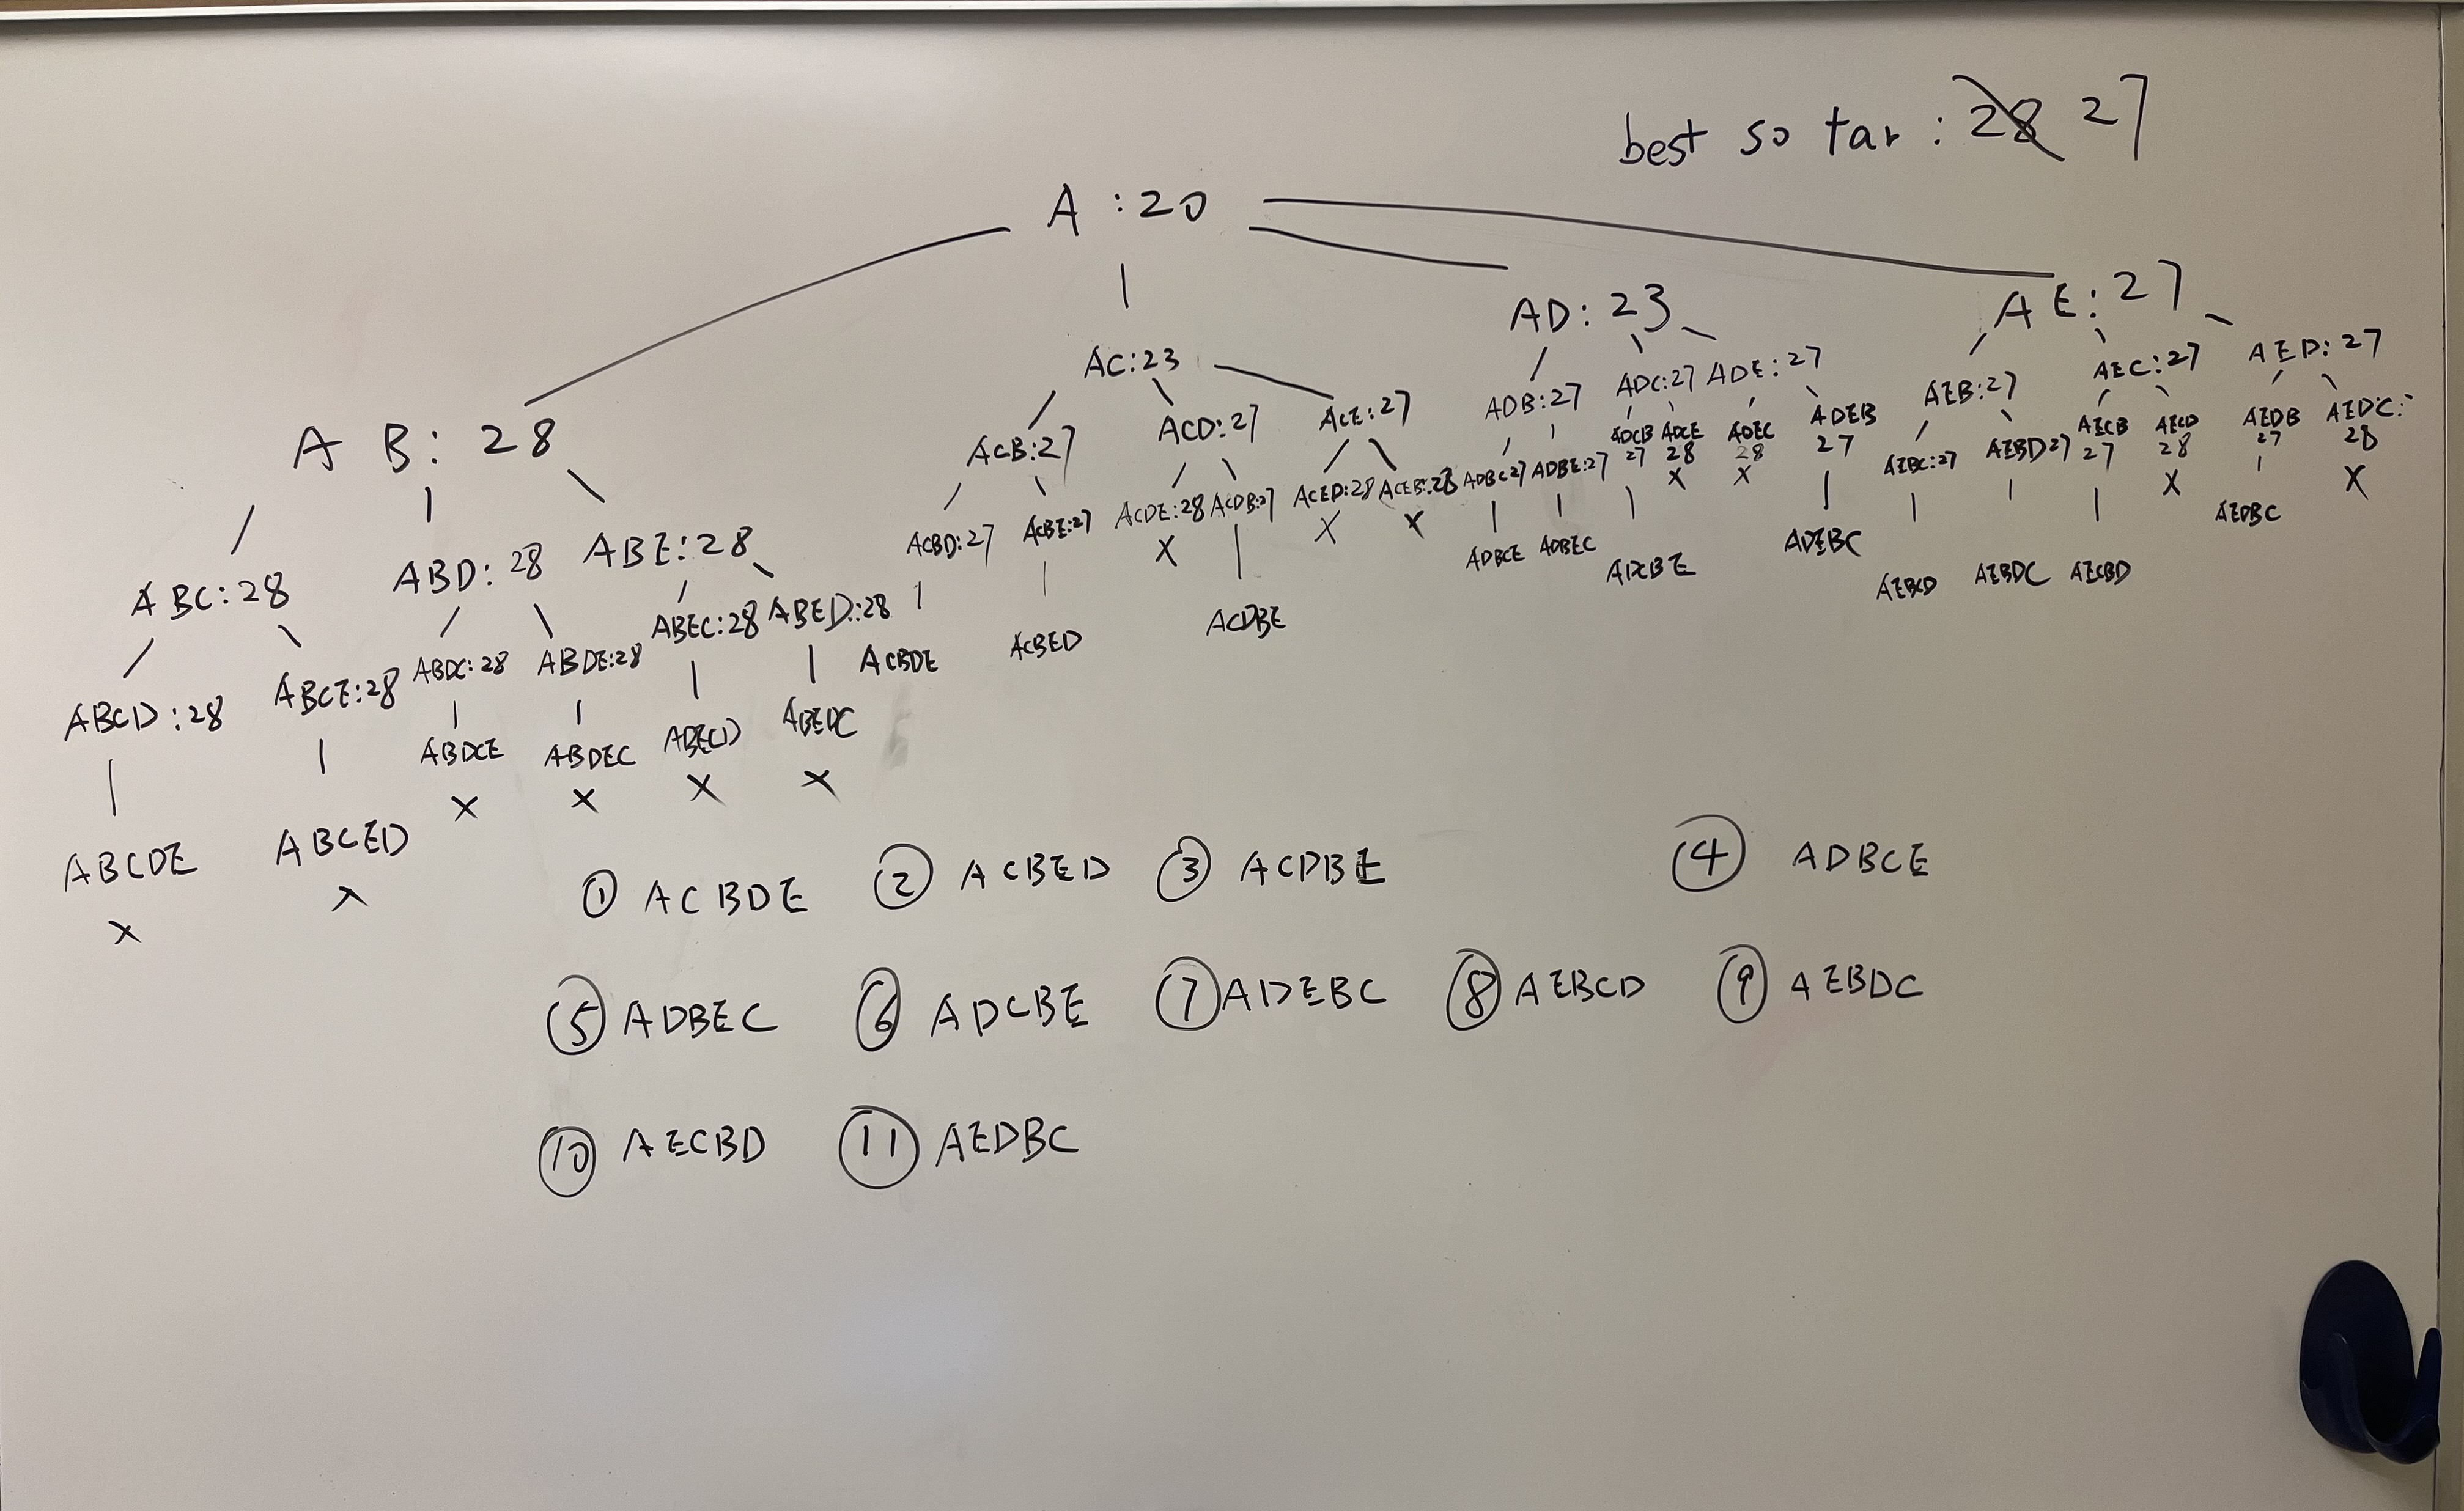
\includegraphics[scale = 0.1]{trees.jpeg}
\end{center}

From my tree, the lower bound for each subproblem is labeled besides and I found the result for
this TSP problem should be 27. 

The process is basically first went trough subproblem AB and get current best which is 28. Then went through AC which I updated current best to 27 and stuck with it to the end.
and currently I found there are 11 ways to get 27.



\begin{lstlisting}
  function e = QR_unshift(A)
    $A_0 = hess(A_0)$
    for k = 1:n (until convergence)
      $Q_kR_k = qr(A_{k-1})$
      $A_k = R_kQ_k$
    end
    e = diag($A_n$)
  end function 

\end{lstlisting}



\begin{lstlisting}
  
  
\end{lstlisting}

\begin{align}
  \mat{Q_1}\mat{R_1} &= \mat{A_0} \nonumber \\
  \mat{A_1} &= \mat{R_1}\mat{Q_1} \nonumber \\
  \mat{A_1} &= \mat{Q_1^{-1}}\mat{Q_1}\mat{R_1}\mat{Q_1} \nonumber \\
  \mat{A_1} &= \mat{Q_1^{-1}}\mat{A_0}\mat{Q_1} \nonumber \\
\end{align}


\begin{align}
  \mat{A_k} &= \mat{R_k}\mat{Q_k} \nonumber \\
  \mat{A_k} &= \mat{Q_k^{-1}}\mat{Q_k}\mat{R_k}\mat{Q_k} \nonumber \\
  \mat{A_k} &= \mat{Q_k^{-1}}\mat{A_{k-1}}\mat{Q_k} \nonumber \\
  \mat{A_k} &= \mat{Q_k^{-1}}\mat{R_{k-1}}\mat{Q_{k-1}}\mat{Q_k} \nonumber \\
  \mat{A_k} &= \mat{Q_k^{-1}}\mat{Q_{k-1}^{-1}}\mat{Q_{k-1}}\mat{R_{k-1}}\mat{Q_{k-1}}\mat{Q_k} \nonumber \\
  \mat{A_k} &= \mat{Q_k^{-1}}\mat{Q_{k-1}^{-1}}\mat{A_{k-2}}\mat{Q_{k-1}}\mat{Q_k} \nonumber \\
\end{align}

\end{document}
